\chapter{Software}
Unterstützen gibt es natürlich für alle Prozessschritte bereits Software. Nachfolgende gehen wir auf drei Softwaregestützte Aspekte ein.

\section{Vorlagen}
Jedes Projekt muss irgendwo anfangen. Um die Konsistenz zwischen den Projekten innerhalb eines Unternehmens zu gewährleisten sind Vorlagen die ideale Lösung. Im Bereich der Webentwicklung bietet sich zum Beispiel Yeoman \cite{yeoman} an. Es handelt sich um eine Community, welche getestete Vorlagen zur Benutzung anbietet. Viele dieser Vorlagen erlaube sogar eine Selektierung bestimmter verwendeter Techniken.

\begin{figure}[!htb]
	\centerline{
\includegraphics[width=0.5\textwidth]{img/yeoman}}
	\caption{Yeoman - THE WEB'S SCAFFOLDING TOOL FOR MODERN WEBAPPS \cite{yeoman}.}
	\label{yeoman}
\end{figure}

\section{Quellverzeichnis}
Essentiell ist ein zentrales Quellverzeichnis in das alle Entwickler ihre Änderungen veröffentlichen. Dazu kann entweder ein internes git oder svn aufgesetzt werden oder ein online verfügbares und etabliertes System. Zu den größten zählen dabei Github \cite{github} und Bitbucket \cite{bitbucket}. Die Unterschiede belaufen sich lediglich auf den öffentlichen oder privaten Nutzen der Quellverzeichnisse.

\section{Automatisches Bauen}
Ist eine Zentrale Verwaltung für den Code vorhanden muss nun noch ein System auf Änderungen horchen und etwas damit durchführen. Für öffentliche Projekte bietet sich Travis CI \cite{travisci} an. Dort können Github Quellverzeichnisse verknüpft und bei Änderungen gebaut werden. Sind es private Angelegenheiten kann ein lokales Jenkins \cite{jenkins} aufgesetzt und genutzt werden. Es bietet ebenfalls das automatische Bauen ist grafisch jedoch nicht so hübsch heraus geputzt wie Travis CI.
\begin{figure}[htb!]
	\subfigure[Travis CI]{
\includegraphics[width=0.49\textwidth]{img/travis-ci}}\hfill
	\subfigure[Jenkins]{
\includegraphics[width=0.49\textwidth]{img/jenkins}}
	\caption{Travis CI  \cite{travisci} und Jenkins \cite{jenkins}}
	\label{travisci-jenkins}
\end{figure}

\section{Codequalität und Tests}
Ist ein eventbasiertes System einsatzbereit kann es mit beliebigen weiteren Tools verknüpft werden. Der größte Fokus liegt oftmals bei Tests und Codequalität. Travis als auch Jenkins unterstützen Unit testing und liefern als Ergebnis aufbereitete Grafiken. Wie viel mit den Tests an Code abgedeckt wird und wie sich sonst um die Qualität des Codes bemüht wurde kann mit z.B. SonarQube \cite{sonarqube} oder Code Climate \cite{code-climate} geprüft werden. Diese Erweiterungen können als böser Finger gesehen werden und weisen die Entwickler auf schlechte Praktiken hin.

\begin{figure}[!htb]
	\centerline{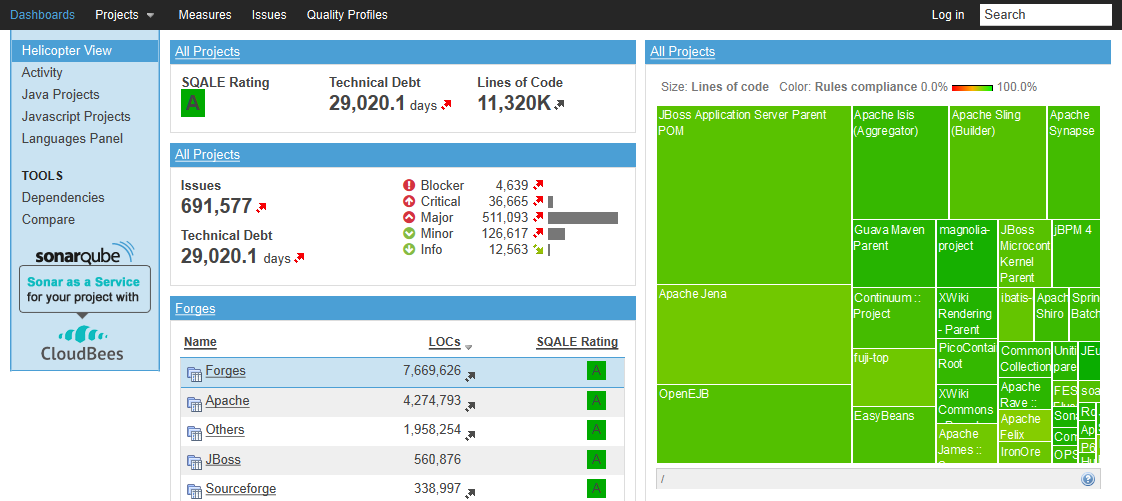
\includegraphics[width=0.5\textwidth]{img/SonarQube}}
	\caption{SonarQube Oberfläche \cite{sonarqube}.}
	\label{sonarqube}
\end{figure}

\begin{figure}[!htb]
	\centerline{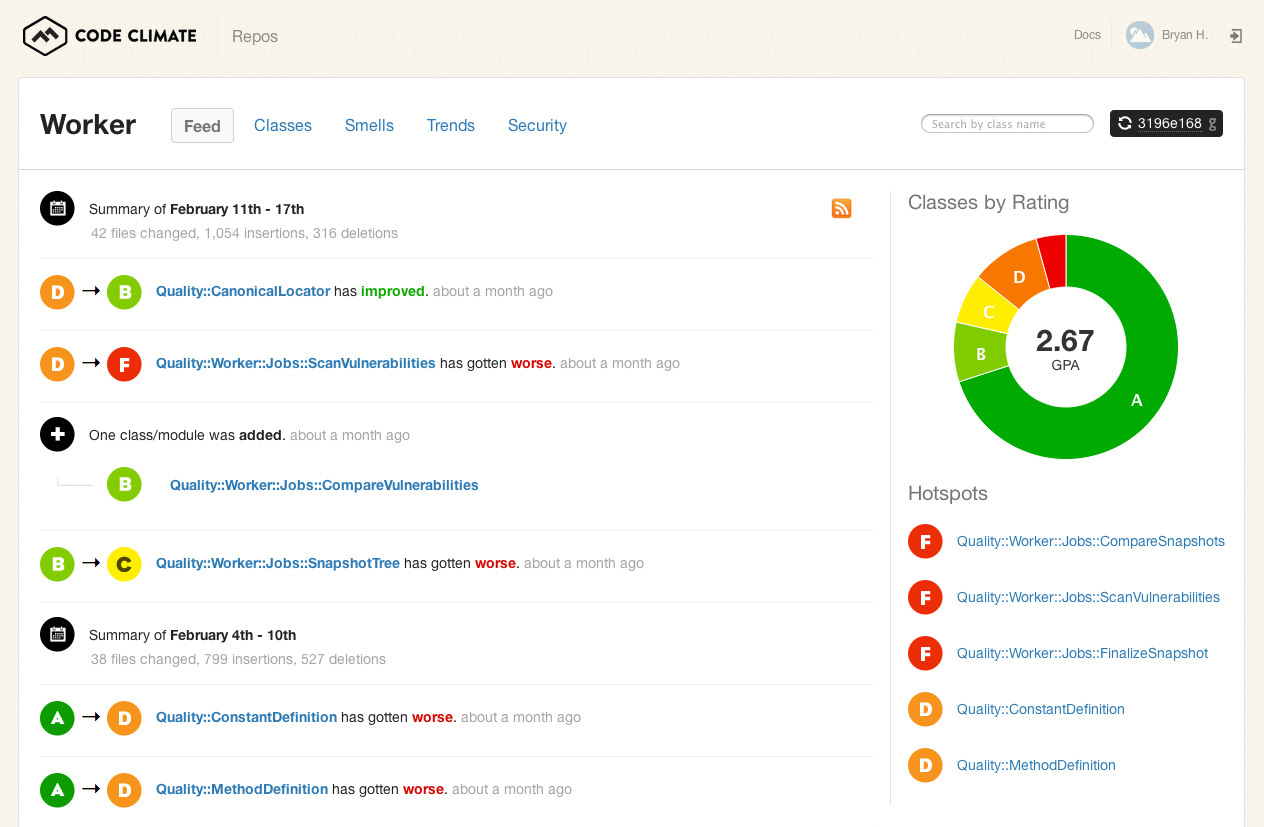
\includegraphics[width=0.5\textwidth]{img/code-climate}}
	\caption{Code Climate Oberfläche \cite{code-climate}.}
	\label{code-climate}
\end{figure}